\section{Features}
\label{sec:approach}

In this section, we describe the features that can be used to measure the word difficulty and these features cover several different aspects including frequency, word length, intra-word, syntactic and semantic features shown in Table \ref{tab:features}.
%We also introduce the model to do the classification of word difficulty.
\begin{table}[ht]
	\centering
	\scriptsize
	\begin{tabular}{lll}
		\hline
		\textbf{Feature}  & \textbf{Description}   \\ \hline
		Frequency        & \tabincell{l}{The number of a words' occurrences in the corpus.}                  \\ 
		Length              & The number of characters in a word                                     \\ \hline
		Phoneme Vector  & The bag-of-phonemes representation of a word                                \\ 
		N-gram Vector            & N-gram transform of a word.                              \\ 
		N-gram Probability    & \tabincell{l}{A probabilistic language model based on \\n-gram at word level.} \\ \hline
		POS Tag              & Word's treebank-specific part-of-speech value.           \\
		%		& uPOS                      & Word's universal part-of-speech value.                   \\ \cline{2-3} 
		Type dependency& \tabincell{l}{Universal dependencies obtained by\\ constituency parsing. }   \\ \hline
		Word embedding       & Pre-trained word vectors.              \\ \hline
	\end{tabular}
	\vspace{-0.25cm}
	\caption{\label{tab:features} Multi-faceted features describing the word difficulty.}
\end{table}
%\subsection{Features}
\label{sec:feature}
%We denote the leveled word set as $\boldmath{W}=\{W_1,\dots,W_K\}$, where K is the number of levels. The vocabulary set extracted from the specific corpus is denoted as V.

\subsection{Frequency and Length}
Frequency and length can't be classified into intra-word, syntactic and semantic features, so they will be talked about individually.

Frequency is a common measurement which is calculated on a huge corpus to assess vocabulary difficulty as mentioned above.
%Several researchers have applied words frequency counts as a means of estimating word difficulties. \JQ{delete "Several...difficulties" }
%We obtain the word frequencies based on a large amount of texts. 
%choosing the frequency index (FI) calculated as $\log_{10}(F+1)$. \JQ{
	The frequency index (FI) is calculated as \begin{equation}
	FI=\log_{10}(F+1)
	\end{equation}  Here, the constant 1 is used to take out-of-corpus words in to computation.
%	prevent minus results for out-of-corpus words.
	
%If one word $w\in \boldmath{W}$ doesn't exist in vocabulary set $\boldmath{V}$ which is generated from a particular corpus, FI of word $w$ will be set as 0.\JQ{Following the equation above, it is zero. So, emmm???}
%In order to avoid confusion with words that appear only once in the corpus, we add one to each word's frequency in which their FI is $\log_{10}2$.\JQ{delete this paragraph}
The length of a word can be obtained directly by counting the number of its characters.

\subsection{Intra-word Features}
%English is a morphological language, whose sounds and spellings of words are corresponding to the morphemes units of English.
%Most languages have morphological features whose sounds and spellings of words are corresponding to the morpheme units.
The difficulty of a word cannot be separated from its intra-word features.
In this part, we use a series of natural language processing (NLP) approaches to obtain the intra-word characters of vocabulary. 
Intuitively, the intra-word features of a word include its spelling rules and pronunciation rules as follows:

\textbf{Pronunciation.} 
%\JQ{maybe need an example for syllables}
%Pronunciation here is the way in which a word is spoken.\JQ{delete "Pronunciation...spoken"} 
In linguistic terminology, phonemes consist of all the distinct units of sounds used by any language, including vowels and consonants.
We use a standard pronunciation dictionary~\cite{John2004CMU}
% CMU Pronunciation Dictionary (CMUdict) 
to generate the phonemes of an English word.
For example, the phonemes of word ``cheese'' are ``CH'', ``IY'' and ``Z''.
A phoneme indicative vector $\mathbf{p_w}=[p_1, p_2, \dots, p_P]$ is set to represent a word's pronunciation, where P is the number of all the phonemes. Set the $i$-th phoneme $p_i=1$ if it exists in a word, otherwise $p_i=0$.
%We only consider the composition of phonemes, ignoring the accent of them when pronuncing a word.\JQ{delete the last sentence?}

\textbf{N-gram Probability.} 
Several researchers and linguists indicated that the spelling regulation of a word may influence its difficulty.
Therefore  we represent each word with its n-gram forms.
Different from traditional language models designed to predict the next word in the sequence of words,  we apply it at character level, which generates the character sequence of a word to capture their stems.

We transform each word into its lower case and add the starting and ending token ``\$" to the word. After that, we get the bigram and trigram froms of words. For example, the bigram combination of word ``x-ray" is (``\$x'',``x-'',``-r'',``ra'',``ay'',``y\$'').
%After retaining those words only containing characters of alphabets and transforming each word into its lower case, there are 26 single letters, from a to z, included in both bigram and trigram forms.
%For example, when the starting and the ending token of a word are also taken into consideration, the bigram combination of word ``a" is (``\$", ``a") and (``a", ``\$") and its trigram combination is (``\$", ``a", ``\$"). 

%We make an \textcolor{red}{assumption} that if the bigrams appeared in a word are seen frequently in the whole corpus, this word is easy to write and remember.
When n-gram model applied at word level, it can be regarded as the probability of forming a word. The greater the probability is, the more fluent the spelling will be. 
Suppose the word $w$ is composed of the character sequence $c_1, c_2, \dots, c_n$, 
%the word-level language model is implemented as follows:
The log probability of the language model is computed as follows:
%\begin{equation}
%\small
%\label{equ:proba}
%\begin{split}
%p(w)&=p(c_1) p(c_2|c_1)\dots p(c_n|c_1,\dots,c_{n-1})\\
%&=p(c_1) p(c_2) \dots  p(c_3)
%\end{split}
%\end{equation}
%Here, the probability of a word is expanded based on the chain rule. Besides, we assume that the probability of each word is independent.
%The Laplace estimate for the probability distribution is applied to generate the n-gram frequency distribution~\cite{field1988laplacian}. 
%It approximates the probability of an n-gram with count $c$ from a collection with $M$ outcomes and $B$ bins as $(c+1)/(M+B)$, which is equivalent to adding 1 to each bin and obtaining the maximum likelihood estimate of the frequency distribution result.
%The probability of a given n-gram is in the range of $[0, 1]$.
%, then the entire word calculated by Formulation \ref{equ:proba} will be even small.\JQ{delete "then...small."}
%To get round this problem we compute the probability of each n-gram as log probability and the bigram and trigram language model implemented at word level is shown as Formulation \ref{equ:bi&tri}.\JQ{ 
%	We compute the log probability of each n-gram to make the figures computable.
%	The formulation is shown as :

\begin{equation}
\small
\label{equ:bi&tri} 
\begin{split}
\log\left(p_{Bi}\right)&=\log\left(p(c_1|``\$")\right)+\log\left(p(c_2|c_1)\right)\\
&+\dots+
%\log\left(p(l_n|l_{n-1})\right)+
\log\left(p(``\$"|c_n)\right)\\
\log\left(p_{Tri}\right)&=\log\left(p(c_2|c_1,``\$")\right)+\log\left(p(c_3|c_2,c_1)\right)\\
&+\dots+\log\left(p(``\$"|c_n,c_{n-1})\right)
\end{split}
\end{equation}

\textbf{N-gram Vector.} 
Different from the probability of entire word calculated by Formulation \ref{equ:bi&tri}, one word can also be represented by its n-gram components which can represent the inflections such as prefixes, suffixes and infixes.
%For the bigram representation of a word, it is a $729$-dimensional ($27\times 27$) vector because the starting and the ending token of word are included in the bigram forms.
%For example, the bigram combination of word ``a" is (``\$", ``a") and (``a",``\$") so that the position of these two bigrams in bigram representation vector can be set 1 and other positions can be set 0.\JQ{delete "a" example}
%For example, the bigrams in word ``the" are (``\$", ``t"), (``t", ``h"), (``h",``e") and (``e", ``\$"), thus the corresponding four positions of its bigram representation vector will be 1.
For one word, the corresponding positions of its n-gram representation vector will be 1.
%\JQ{I think this example can be deleted}
%Similarly the trigram representation of one word is a binary vector in larger size and each trigram segment is obtained by dividing the original word by length 3.
Figure \ref{fig:bitri} indicates the n-gram combinations and vectors in which 1 stands for an n-gram appears in the corresponding position and the dots in each vector means 0.
\begin{figure}[th]
	\centering
	\scriptsize
%	\epsfig{file=pic/bitri.eps, width=0.9\columnwidth}
	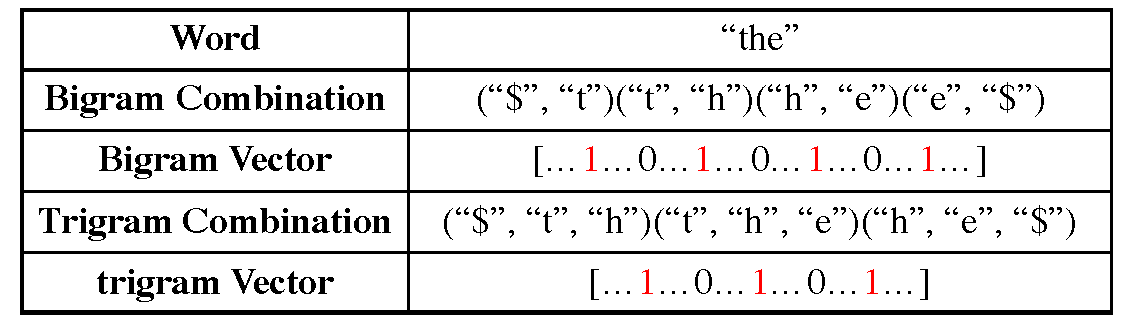
\includegraphics[width=1\linewidth]{pic/bitri.pdf}  
	\vspace{-0.45cm}
	%\caption{Overview of proposed model, which shows how Attention Filter Mechanism (ATTF) works when decoding $Y_i$.}
	\caption{Examples of Bigram and Trigram Vectors.}
	\label{fig:bitri}
\end{figure}
\vspace{-0.5cm}
\subsection{Syntactic Features}
The use of words can't be cut off from sentences. 
Intuitively, the difficulty of a word may be related to its role 
%in the sentence\JQ{delete "in the sentence"} 
and the relation with other words appearing in the sentence.
In this section, we apply the part-of-speech (POS) tagging~\cite{toutanova2003feature} and universal dependencies representation~\cite{schuster2016enhanced} obtained by Stanford CoreNLP to generate these features. 
These two are used to  reflect the syntactic features of a word.

\textbf{POS Tag.} A binary indicative vector is selected to indicate the POS tag feature.
% and universal dependencies.
%For example, $T$-dimension POS vector $\mathbf{t_w}=[t_1, t_2,\dots, t_T]$ for word $w\in \boldmath{W}$ is the representation of  $T$ types of POS taggers marked in the documents. 
%The $i$-th element of vector $\mathbf{t_w}$ marked 1 indicates that the word $w$ has the $i$-th POS in the text. 
A $T$-dimension POS vector $\mathbf{t_w}=[t_1, t_2,\dots, t_T]$ is designed for each word, where $T$ represents the number of different POS tags. The $i$-th element of vector $\mathbf{t_w}$ marked 1 indicates that the word $w$ exists the $i$-th POS in the text.

\textbf{Universal Dependencies.}
%Vector of universal dependency follows the similar principle.\JQ{
	The vector of universal dependency follows the similar principle.
Figure \ref{fig:parser} shows an example of a parsing result obtained by Stanford CoreNLP\footnote{An online application of Stanford parser: \url{http://corenlp.run/}}.

In order to represent the universal dependencies of each word into a vector, we considered the direction of each type.
%\JQ{lack of explanation for direcction}
%Add ``\_in" to the word's relationship which the arrow points to and add ``\_out" to the relationship which the arrow points out.
Add ``\_in" after the word's relationship which is pointed to this word and add ``\_out" after the relationship which is pointed out from the word.
For the example in Figure \ref{fig:parser}, 
word ``man" has the dependencies of ``amod\_out'', ``det\_out'', ``cop\_out'', ``nsubj\_out'' and ``punct\_out''.
While word ``He'' has the dependency of ``nsubj\_in".
Then we use the types of dependencies appeared in the documents to generate the bags as the words' dependencies representation whose binary vector form is similar to Figure \ref{fig:bitri}.
\begin{figure}[th]
	\centering
	%	\epsfig{file=pic/bitri.eps, width=0.9\columnwidth}
	\includegraphics[width=1\linewidth]{pic/parsing.eps} 
	\vspace{-0.25cm}
	\caption{Parsing result for sentence ``He is a handsome man." obtained by Stanford CoreNLP parser.}
	\label{fig:parser}
\end{figure}

\subsection{Semantic Features}
The difficulty of a word is also related to its meanings.
However, the semantic knowledge of a word is not only rely on itself but also reflected by its context. 
Therefore, we utilize word embeddings to represent each word appearing in the documents and capture its syntactic and semantic features, including the word similarity, synonym and topical information.

%Word2Vec and GloVe are both useful technique to learn word embedding and generate a fixed vector representation of a particular word. 
%In other to take the polysemy into consideration, the contextualized embedding such as BERT is also be chosen as a means to represent the word. 
%Different from the tasks at sentence level, we don't need any sentence representation but the word embeddings after training the BERT model.

%\subsection{Classification and Word Pairs Difficulty Ranking}
%Based on the extracted features mentioned in Section \ref{sec:feature}, we implement both the classification model and pairs difficulty ranking model to measure the word difficulty.
%In this part, we will try support vector machine (SVM), logistic regression (LR) and multi-layer perceptron (MLP) and pick the model with the best results.
%To compare the difficulty of any two words, we implement word pairs difficulty ranking.

%During the training state of MLP, we choose a three-layer neural network and update the parameters by iteratively sampling one mini-batch from dataset.
%Considering the lack of training samples and large feature dimensions, we choose linear kernel or optimization algorithm in SVM and LR.
